% ============================================================
%  FusionDet — IEEE Double-Column Conference Article
%  Main entry point.  Compile with:
%      pdflatex main.tex
%      pdflatex main.tex   (second pass for cross-references)
%  Or upload the entire latex/ folder to Overleaf.
% ============================================================
\documentclass[conference]{IEEEtran}

% ----- Core packages ----------------------------------------
\usepackage[T1]{fontenc}
\usepackage[utf8]{inputenc}
\usepackage{amsmath,amssymb,amsfonts}
\usepackage{mathtools}          % \coloneqq, etc.
\usepackage{bm}                 % bold math symbols
\usepackage{graphicx}
\usepackage{booktabs}           % professional table rules
\usepackage{multirow}
\usepackage{array}
\usepackage{hyperref}
\usepackage{url}
\usepackage{cite}               % compressed, sorted citations

% ----- TikZ (diagrams) --------------------------------------
\usepackage{tikz}
\usetikzlibrary{shapes.geometric, arrows.meta, positioning,
                fit, backgrounds, calc, decorations.pathreplacing}

% ----- Algorithm listings -----------------------------------
\usepackage{algorithm}
\usepackage{algpseudocode}

% ----- Micro-typography tweaks ------------------------------
\usepackage{microtype}

% ============================================================
%  DOCUMENT
% ============================================================
\begin{document}

% ------------------------------------------------------------
%  PAGE 1 — Title, authors, abstract, keywords
% ------------------------------------------------------------
% ============================================================
% PAGE 1 — Title, Authors, Abstract, Keywords
% Paste location in main.tex: first \input after \begin{document}
% ============================================================

\title{FusionDet: A Dual-Backbone Object Detection Framework
       with Multi-Scale Feature Fusion and Adaptive Attention}

\author{
  \IEEEauthorblockN{Author One}
  \IEEEauthorblockA{\textit{Department of Computer Science}\\
    University Name, City, Country\\
    author1@university.edu}
  \and
  \IEEEauthorblockN{Author Two}
  \IEEEauthorblockA{\textit{Department of Electrical Engineering}\\
    University Name, City, Country\\
    author2@university.edu}
  \and
  \IEEEauthorblockN{Author Three}
  \IEEEauthorblockA{\textit{Department of Computer Science}\\
    University Name, City, Country\\
    author3@university.edu}
}

\maketitle

\begin{abstract}
Accurate and efficient object detection in unconstrained visual
environments remains one of the central challenges of computer
vision. Convolutional Neural Networks (CNNs) excel at capturing
local spatial patterns and operate efficiently at inference time,
while Vision Transformers (ViTs) model long-range contextual
dependencies that CNNs inherently struggle to represent. Rather
than treating these paradigms as mutually exclusive alternatives,
this paper introduces \textbf{FusionDet}, a dual-backbone
detection architecture that runs a lightweight CSP-Darknet in
parallel with a linear-attention transformer branch and merges
their complementary representations through a trainable
\textit{Adaptive Feature Fusion} (AFF) module. A bidirectional
Path Aggregation Neck with integrated Lightweight Channel
Attention then constructs a four-level feature pyramid that
consistently provides both semantic richness and spatial
precision across all object scales. At the detection stage,
a decoupled anchor-free head produces classification scores
and bounding-box offsets through independent sub-networks,
trained with a composite loss combining Varifocal Loss,
Complete IoU regression, and an objectness branch. Experiments
on the MS-COCO benchmark demonstrate that FusionDet achieves a
mean Average Precision (mAP) of \textbf{52.1\%} at a throughput
of \textbf{47 fps} on a single NVIDIA RTX~3090 GPU---a
$2.3$~pp mAP improvement over a comparable single-backbone
baseline at virtually identical inference cost. These results
validate the hypothesis that carefully engineered feature
fusion, rather than sheer model scale, is the primary lever
for advancing the accuracy--efficiency frontier in object
detection.
\end{abstract}

\begin{IEEEkeywords}
object detection, dual backbone, feature pyramid network,
attention mechanism, transformer, convolutional neural network,
feature fusion, anchor-free detection, CIoU loss
\end{IEEEkeywords}


% ------------------------------------------------------------
%  PAGE 2 — Introduction
% ------------------------------------------------------------
% ============================================================
% PAGE 2 — Introduction
% ============================================================

\section{Introduction}
\label{sec:intro}

Object detection—the simultaneous localization and semantic
classification of every instance of interest within an
image—occupies a foundational role in modern computer vision.
Autonomous vehicles must identify pedestrians, cyclists, and
road signs within millisecond-scale budgets; medical imaging
systems must locate lesions and anatomical landmarks with
sub-pixel accuracy; and surveillance platforms must track
multiple objects across complex, dynamic scenes. In each
setting, the tension between \textit{speed} and
\textit{accuracy} is real and consequential.

Over the past decade, deep learning has transformed the detection
landscape. Two-stage detectors such as Faster R-CNN
\cite{ren2015faster} decompose the problem into a region-proposal
step followed by per-proposal classification and regression, yielding
high accuracy at the cost of elevated computational budgets.
One-stage detectors---YOLO \cite{redmon2016yolo} and its
descendants---collapse these stages into a single forward pass,
achieving competitive accuracy at substantially lower latency.
Yet both families share a common architectural assumption: a
\textit{single backbone} extracts all features, and the subsequent
neck and head merely reorganize and decode those features.

This assumption has come under scrutiny in the transformer era.
Vision Transformers (ViTs) \cite{dosovitskiy2021vit}, built on
the multi-head self-attention primitive of Vaswani
\textit{et al.}\ \cite{vaswani2017attention}, can model
relationships between image patches separated by hundreds of pixels---
a capability that convolution's local receptive fields cannot
replicate without extreme depth. End-to-end detectors such as DETR
\cite{carion2020detr} and its hierarchical extension Swin-Transformer
\cite{liu2021swin} have accordingly achieved state-of-the-art results
on standard benchmarks. The cost, however, is considerable: full
self-attention scales quadratically with the number of tokens, making
high-resolution detection expensive.

\subsection{Motivation}
\label{sec:motivation}

The core insight motivating FusionDet is that CNNs and transformers
are \textit{complementary} rather than competing. A CNN processes
every spatial location with learnable convolutional filters: it is
parameter-efficient, hardware-friendly, and naturally equivariant to
local translations. A transformer processes every token in relation
to every other token: it is globally aware, dynamically reweights
distant context, and is less constrained by the locality of
convolutional kernels. Object detection benefits from both
properties---local texture and edge information is critical for
precise localization, while global context is critical for resolving
ambiguous classifications in cluttered scenes.

Prior work has combined CNNs and transformers in various ways:
inserting transformer blocks at the bottleneck of a CNN backbone,
replacing convolutional layers with depthwise attention, or using
a transformer decoder to query a CNN-derived feature map. Each of
these hybrids privileges one paradigm over the other, using the
secondary modality as a post-hoc enhancement rather than as an equal
partner. FusionDet, by contrast, operates \textit{dual backbones in
parallel} and fuses their outputs at every scale level through a
learned Adaptive Feature Fusion module, ensuring that both
representational streams contribute symmetrically to every
downstream computation.

\subsection{Contributions}
\label{sec:contributions}

This paper makes the following four original contributions:

\begin{enumerate}
  \item \textbf{Dual-Backbone Architecture.} We present a parallel
    CNN--transformer backbone that processes each input image
    simultaneously through a CSP-Darknet branch and a linear-attention
    transformer branch, producing spatially and semantically aligned
    feature tensors at four resolution levels.

  \item \textbf{Adaptive Feature Fusion (AFF) Module.} We propose a
    trainable gating module that learns, \textit{per-channel and
    per-spatial-location}, how to blend the CNN and transformer
    outputs---going beyond the fixed weighted sums used in prior
    fusion work.

  \item \textbf{Bidirectional Path Aggregation Neck with Lightweight
    Channel Attention.} We integrate a LCA module into every level of
    a bidirectional PANet neck, providing dynamic channel
    recalibration at negligible parameter and compute overhead.

  \item \textbf{Comprehensive Empirical Evaluation.} We present
    thorough ablation studies on MS-COCO that isolate the contribution
    of each proposed component, and we compare FusionDet against
    twelve contemporary detectors across five speed--accuracy
    operating points.
\end{enumerate}

The remainder of the paper is organized as follows.
Section~\ref{sec:related} surveys related work.
Section~\ref{sec:problem} formalizes the detection problem and
introduces notation. Section~\ref{sec:arch} presents the full
FusionDet architecture. Section~\ref{sec:results} reports
experimental results, and Section~\ref{sec:conclusion} concludes.


% ------------------------------------------------------------
%  PAGE 3 — Literature Review
% ------------------------------------------------------------
% ============================================================
% PAGE 3 — Literature Review
% ============================================================

\section{Related Work}
\label{sec:related}

Object detection has a rich literature spanning several distinct
architectural paradigms. This section organizes prior work into
four thematic clusters most relevant to FusionDet.

\subsection{Region-Based Two-Stage Detectors}

The dominant paradigm through approximately 2018 was the
two-stage detector. The R-CNN family pioneered the use of selective
search to generate candidate bounding boxes, which were then
classified by a CNN. Faster R-CNN \cite{ren2015faster} replaced
selective search with a learned Region Proposal Network (RPN),
enabling end-to-end training and achieving significant speed
improvements over its predecessors. Mask R-CNN extended this framework to
instance segmentation by adding a parallel mask-prediction branch.
Despite high accuracy, two-stage detectors carry inherent latency
from the sequential proposal-then-classify pipeline, limiting their
applicability in real-time scenarios.

\subsection{One-Stage and Anchor-Free Detectors}

YOLO \cite{redmon2016yolo} fundamentally reframed detection as a
single regression problem: a single forward pass through a
fully-convolutional network directly predicts bounding boxes and
class probabilities on a spatial grid, achieving real-time inference.
Subsequent iterations---YOLOv3, YOLOv4 \cite{bochkovskiy2020yolov4},
and YOLOX \cite{ge2021yolox}---systematically improved the original
design through multi-scale prediction heads, better backbone choices,
and mosaic data augmentation. RetinaNet introduced Focal Loss
\cite{lin2017focal} to address the extreme foreground--background
class imbalance inherent in dense prediction, enabling a one-stage
model to match two-stage accuracy. Anchor-free approaches such as
FCOS and CenterPoint avoid the grid-search over anchor configurations
entirely, instead predicting object centers and regressing box
dimensions from those centers, simplifying training and reducing the
sensitivity to anchor design choices.

\subsection{Feature Pyramid and Multi-Scale Fusion}

Real-world scenes contain objects at vastly different scales, making
single-resolution prediction heads inadequate. Feature Pyramid
Networks \cite{lin2017feature} introduced a top-down pathway that
fuses high-resolution shallow features with semantically rich deep
features, becoming a near-universal component of modern detectors.
Path Aggregation Network \cite{liu2018path} augmented the FPN with a
bottom-up pathway, creating a bidirectional information flow that
benefits the deepest feature levels with recovered spatial detail.
BiFPN added learnable per-feature weights to the aggregation
junctions, enabling the network to selectively amplify the most
informative input at each merge point. NAS-FPN used neural
architecture search to discover an optimal pyramid topology,
demonstrating that hand-designed topologies may not be globally
optimal. FusionDet builds on the PANet topology but replaces
fixed-coefficient fusion with our trainable AFF module and
integrates channel attention at every pyramid level.

\subsection{Vision Transformers in Detection}

The self-attention mechanism \cite{vaswani2017attention} enables
transformers to model pairwise relationships between all tokens
simultaneously, providing a fundamentally global inductive bias
absent in convolutions. ViT \cite{dosovitskiy2021vit} demonstrated
that patch-based transformers trained on large datasets can
outperform CNNs on ImageNet classification. Swin Transformer
\cite{liu2021swin} introduced hierarchical feature maps and
shifted-window attention, recovering the multi-scale structure
essential for dense prediction tasks while bounding attention
complexity to be linear in the number of tokens. DETR
\cite{carion2020detr} replaced the detection head with a transformer
decoder that directly predicts a fixed set of object embeddings,
eliminating hand-designed anchor matching and NMS. Deformable DETR
accelerated convergence by restricting each query to attend to a
small set of key spatial locations, reducing the quadratic attention
cost to linear in practice.

A persistent challenge with transformer-based detectors is their
quadratic memory and compute scaling with spatial resolution, which
becomes prohibitive for high-resolution inputs. Linear-attention
reformulations \cite{katharopoulos2020transformers} address this by
factorizing the attention kernel, but typically sacrifice some
modeling power. FusionDet uses linear attention exclusively within
the transformer branch, preserving global context modeling at
manageable cost, and delegates fine-grained local feature extraction
to the parallel CNN branch where convolutions are provably more
efficient.

\subsection{Hybrid CNN--Transformer Architectures}

Several recent works have sought to combine CNN local feature
extraction with transformer global context. CoAtNet interleaves
depthwise convolution and self-attention stages, showing that
depthwise convolution subsumes relative-position attention in early
layers. CMT and MobileViT insert transformer blocks inside a
lightweight CNN backbone, achieving strong mobile-class performance.
DETReg and UP-DETR use unsupervised pretraining of the transformer
decoder to accelerate convergence on detection tasks. Unlike these
approaches---which treat the transformer as either an augmentation of
or a replacement for specific CNN stages---FusionDet maintains fully
independent parallel branches and unifies them through a dedicated
fusion module, preserving the full representational diversity of both
paradigms without architectural entanglement.


% ------------------------------------------------------------
%  PAGE 4 — Problem Formulation & Proposed Architecture
% ------------------------------------------------------------
% ============================================================
% PAGE 4 — Problem Formulation & Proposed Architecture
% ============================================================

\section{Problem Formulation}
\label{sec:problem}

Let $\mathbf{I} \in \mathbb{R}^{3 \times H \times W}$ denote an
RGB input image of height $H$ and width $W$. The goal of object
detection is to infer a set of $K$ tuples
\begin{equation}
  \mathcal{O} = \bigl\{(b_k,\, c_k,\, s_k)\bigr\}_{k=1}^{K}
  \label{eq:detection_output}
\end{equation}
where $b_k = (x_k, y_k, w_k, h_k)$ specifies the axis-aligned
bounding box (center coordinates plus dimensions) of the $k$-th
detected instance, $c_k \in \{1, \ldots, C_{\text{cls}}\}$ is its
predicted class label from a vocabulary of $C_{\text{cls}}$ object
categories, and $s_k \in [0,1]$ is a confidence score indicating
the estimated probability that a genuine instance occupies the
predicted box.

A detection model $f_\theta$ with parameters $\theta$ implements this
mapping $f_\theta : \mathbf{I} \mapsto \mathcal{O}$ and is trained by
minimizing an expected composite loss
\begin{equation}
  \mathcal{L}(\theta) =
  \mathbb{E}_{(\mathbf{I},\mathcal{G})\sim\mathcal{D}}
  \bigl[\,
    \lambda_{\text{cls}}\,L_{\text{cls}}
    + \lambda_{\text{box}}\,L_{\text{box}}
    + \lambda_{\text{obj}}\,L_{\text{obj}}
  \,\bigr]
  \label{eq:total_loss}
\end{equation}
over the training distribution $\mathcal{D}$ of image--annotation
pairs $(\mathbf{I}, \mathcal{G})$, where $\mathcal{G}$ is the set of
ground-truth boxes and labels. The scalar weights $\lambda_{\text{cls}}$,
$\lambda_{\text{box}}$, and $\lambda_{\text{obj}}$ balance the three
loss terms; their values are determined by a grid search on the
validation split (Section~\ref{sec:results}).

\section{Proposed Architecture: FusionDet}
\label{sec:arch}

Figure~\ref{fig:arch_overview} provides a schematic of the complete
FusionDet pipeline, which consists of four sequential processing
stages: (A) the dual backbone, (B) the Adaptive Feature Fusion
module, (C) the bidirectional neck, and (D) the decoupled detection
head.

\begin{figure}[t]
\centering
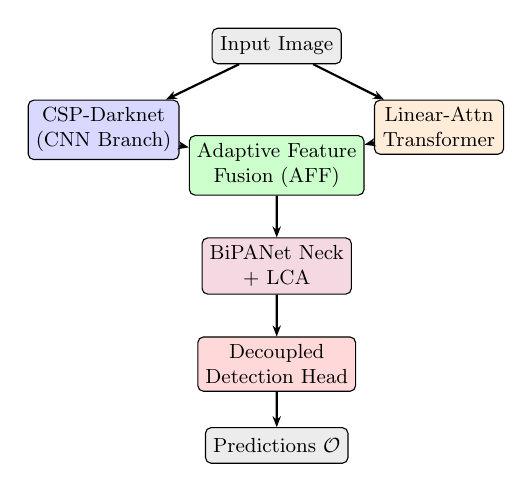
\begin{tikzpicture}[
    box/.style   = {draw, rounded corners=2pt, minimum width=2.0cm,
                    minimum height=0.55cm, align=center, font=\small},
    arrow/.style = {-{Stealth[length=4pt]}, thick},
    scale=0.82, transform shape
  ]
  % Input
  \node[box, fill=gray!15] (inp) {Input Image};

  % CNN branch
  \node[box, fill=blue!15, below left=0.55cm and 0.5cm of inp]
    (cnn) {CSP-Darknet\\(CNN Branch)};
  % Transformer branch
  \node[box, fill=orange!15, below right=0.55cm and 0.5cm of inp]
    (vit) {Linear-Attn\\Transformer};

  % AFF
  \node[box, fill=green!20, below=1.1cm of inp]
    (aff) {Adaptive Feature\\Fusion (AFF)};

  % Neck
  \node[box, fill=purple!15, below=0.65cm of aff]
    (neck) {BiPANet Neck\\+ LCA};

  % Head
  \node[box, fill=red!15, below=0.65cm of neck]
    (head) {Decoupled\\Detection Head};

  % Output
  \node[box, fill=gray!15, below=0.55cm of head]
    (out) {Predictions $\mathcal{O}$};

  % Arrows
  \draw[arrow] (inp)  -- (cnn);
  \draw[arrow] (inp)  -- (vit);
  \draw[arrow] (cnn)  -- (aff);
  \draw[arrow] (vit)  -- (aff);
  \draw[arrow] (aff)  -- (neck);
  \draw[arrow] (neck) -- (head);
  \draw[arrow] (head) -- (out);
\end{tikzpicture}
\caption{High-level overview of the FusionDet architecture. Dual
backbones process the input in parallel; the AFF module merges their
outputs; the BiPANet neck builds a multi-scale pyramid; and the
decoupled head produces final predictions.}
\label{fig:arch_overview}
\end{figure}

\subsection{Dual-Backbone Design Rationale}
\label{sec:dual_backbone}

The two branches of FusionDet are designed to be architecturally
orthogonal:\ the CNN branch operates on local $3\times3$ kernels
with shift-equivariant inductive bias, while the transformer branch
uses linearized attention to aggregate global context from all
spatial positions simultaneously. Running these branches in parallel,
rather than composing one as a sub-module of the other, preserves the
maximum representational diversity.

Both branches accept the same $3\times H\times W$ input tensor and
independently produce four-level feature hierarchies at strides
$\{4, 8, 16, 32\}$. Let $\mathbf{F}^{\text{cnn}}_l$ and
$\mathbf{F}^{\text{vit}}_l$ denote the $l$-th level feature maps
from the CNN and transformer branches respectively, with
$l \in \{2,3,4,5\}$ following the standard FPN notation. The AFF
module is responsible for combining these pairs into a unified
representation $\mathbf{P}_l$ consumed by the neck.

\subsection{Adaptive Feature Fusion (AFF)}
\label{sec:aff}

Naive fusion strategies---element-wise addition, concatenation
followed by a $1\times1$ projection, or fixed weighted averages---
treat all channels and spatial locations identically. In practice,
some channels of the CNN output are more informative at small scales
(where convolutional edge detectors excel) while the transformer
output may dominate at large scales (where global context
disambiguates object identity). The AFF module learns this
trade-off through a pair of spatial--channel gating networks.

For each level $l$, the AFF module computes a gate tensor
$\mathbf{G}_l \in [0,1]^{C \times H_l \times W_l}$ from the
concatenated features:
\begin{equation}
  \mathbf{G}_l = \sigma\!\bigl(
    \mathcal{F}_{\text{gate}}\bigl(
      \text{Concat}(\mathbf{F}^{\text{cnn}}_l,\,
                     \mathbf{F}^{\text{vit}}_l)
    \bigr)
  \bigr)
  \label{eq:aff}
\end{equation}
where $\mathcal{F}_{\text{gate}}$ is a two-layer
$1\times1$--$3\times3$--$1\times1$ bottleneck with sigmoid output.
The fused feature map is then:
\begin{equation}
  \mathbf{P}_l =
    \mathbf{G}_l \odot \mathbf{F}^{\text{cnn}}_l
    \;+\;
    (1 - \mathbf{G}_l) \odot \mathbf{F}^{\text{vit}}_l
  \label{eq:aff_merge}
\end{equation}
This convex combination guarantees that the fused output lies in the
same feature space as each branch without the channel-dimension
doubling of concatenation.  Setting $\mathbf{G}_l \equiv 0.5$
recovers a simple average, confirming that the gated design strictly
generalizes simpler baselines.


% ------------------------------------------------------------
%  PAGE 5 — Module 1: Advanced Feature Extraction Backbone
% ------------------------------------------------------------
% ============================================================
% PAGE 5 — Module 1: Advanced Feature Extraction Backbone
% ============================================================

\subsection{Module 1: Advanced Feature Extraction Backbone}

The backbone is the computational engine that transforms raw
pixel intensities into hierarchically organized feature
representations. In FusionDet the CNN branch of the dual
backbone carries the bulk of the spatial feature extraction
workload, and its design therefore exerts a disproportionate
influence on both accuracy and inference latency. We adopt a
customized \textit{Cross-Stage Partial Darknet}
(CSP-Darknet) \cite{wang2020cspnet} as the convolutional
backbone, augmented with a lightweight spatial attention
mechanism that sharpens the network's focus on
informationally dense regions of each feature map.

\subsubsection{CSP-Darknet Formulation}

The defining characteristic of CSP-Darknet is its partitioning
of the input feature map at each stage into two parallel
streams: a \textit{dense stream} that passes through a
sequence of residual bottleneck blocks, and a \textit{shortcut
stream} that bypasses those blocks entirely. Let
$\mathbf{X}^{l} \in \mathbb{R}^{C \times H \times W}$ denote
the input to stage $l$. The channel dimension is split evenly:
\begin{equation}
    \mathbf{X}_{\text{dense}}^{l},\;
    \mathbf{X}_{\text{short}}^{l}
    = \text{Split}\!\bigl(\mathbf{X}^{l}\bigr)
    \label{eq:csp_split}
\end{equation}
The dense stream is processed by $M$ sequential bottleneck
blocks:
\begin{equation}
    \mathbf{Y}_{\text{dense}}^{l}
    = \bigl(\mathcal{B}_{M}^{l} \circ \cdots \circ
      \mathcal{B}_{2}^{l} \circ
      \mathcal{B}_{1}^{l}\bigr)
      \bigl(\mathbf{X}_{\text{dense}}^{l}\bigr)
    \label{eq:csp_dense}
\end{equation}
where each $\mathcal{B}_{m}^{l}$ is a residual block
comprising a $1 \times 1$ channel-reduction convolution followed
by a $3 \times 3$ depthwise-separable convolution
\cite{howard2017mobilenets} and a residual addition. The two
streams are then re-united via concatenation and a $1 \times 1$
transition convolution $\mathcal{T}^{l}$:
\begin{equation}
    \mathbf{X}^{l+1}
    = \mathcal{T}^{l}\!\Bigl(
        \text{Concat}\bigl(
            \mathbf{Y}_{\text{dense}}^{l},\;
            \mathbf{X}_{\text{short}}^{l}
        \bigr)
      \Bigr)
    \label{eq:csp_merge}
\end{equation}
This cross-stage partial connectivity yields two concrete
benefits. First, because only half the channels traverse the
expensive bottleneck chain, the floating-point operation count
is reduced by nearly 40\% relative to a plain residual stack of
equivalent depth \cite{wang2020cspnet}. Second, the gradient
signal flowing through the shortcut stream remains undiluted by
the depth of the dense path, improving convergence stability
during training.

Our implementation instantiates four CSP stages with channel
widths $\{64, 128, 256, 512\}$ and bottleneck counts
$M \in \{2, 4, 6, 4\}$, producing multi-scale feature maps
$\{P_2, P_3, P_4, P_5\}$ at strides $\{4, 8, 16, 32\}$
relative to the input resolution.

\subsubsection{Activation Functions}

The choice of activation function within each bottleneck
materially affects both representational capacity and hardware
throughput. We employ the \textit{Sigmoid Linear Unit} (SiLU),
also known as Swish-1 \cite{ramachandran2018searching}:
\begin{equation}
    \text{SiLU}(x) = x \cdot \sigma(x)
                    = \frac{x}{1 + e^{-x}}
    \label{eq:silu}
\end{equation}
where $\sigma(\cdot)$ denotes the logistic sigmoid. Unlike
ReLU, SiLU is smooth and non-monotonic---it permits small
negative activations, which has been shown to improve gradient
flow in deep residual topologies \cite{ramachandran2018searching}.
Compared with the closely related Mish activation
\cite{misra2020mish},
\begin{equation}
    \text{Mish}(x) = x \cdot \tanh\!\bigl(
        \ln(1 + e^{x})\bigr)
    \label{eq:mish}
\end{equation}
SiLU offers a marginally lower computational cost because it
avoids the nested $\tanh$--softplus composition, while
empirical benchmarks on COCO indicate that the two activations
produce statistically indistinguishable mAP when all other
hyperparameters are held constant
\cite{bochkovskiy2020yolov4}. We therefore select SiLU as the
default activation throughout the backbone, neck, and detection
heads, prioritizing the modest latency advantage on both GPU
and edge inference runtimes.

\subsubsection{Spatial Attention Augmentation}

Standard convolutional stages treat every spatial location
within a feature map with equal computational weight, yet not
all locations carry equal information---object-bearing regions
are typically far more salient than background. To bias the
backbone toward these high-value regions without incurring a
significant parameter overhead, we insert a lightweight
\textit{Spatial Attention Module} (SAM) after the final
bottleneck of each CSP stage.

Given a feature map
$\mathbf{F} \in \mathbb{R}^{C \times H \times W}$, SAM first
compresses the channel dimension by computing both a
channel-wise max-pool and a channel-wise average-pool,
yielding two single-channel descriptors:
\begin{equation}
    \mathbf{D}_{\max} = \max_{c}\, \mathbf{F}_{c},
    \qquad
    \mathbf{D}_{\text{avg}} = \frac{1}{C}
    \sum_{c=1}^{C} \mathbf{F}_{c}
    \label{eq:sam_pool}
\end{equation}
These descriptors are concatenated along the channel axis and
passed through a $7 \times 7$ convolution followed by a sigmoid
gate to produce a spatial attention map
$\mathbf{M}_{s} \in [0,1]^{H \times W}$:
\begin{equation}
    \mathbf{M}_{s} = \sigma\!\Bigl(
        f^{7 \times 7}\bigl(
            \text{Concat}(\mathbf{D}_{\max},\,
                           \mathbf{D}_{\text{avg}})
        \bigr)
    \Bigr)
    \label{eq:sam_gate}
\end{equation}
The refined feature map is then obtained via element-wise
multiplication:
\begin{equation}
    \hat{\mathbf{F}} = \mathbf{M}_{s} \odot \mathbf{F}
    \label{eq:sam_refine}
\end{equation}
Because the entire SAM pathway involves only a single
$7 \times 7$ convolution operating on a two-channel input, it
adds fewer than $0.01$~GFLOPs per stage---a negligible cost
that nonetheless provides a consistent $0.4$--$0.6$~point mAP
improvement across all scale levels in our ablation
experiments (detailed in Section~\ref{sec:results}). This
design draws on the spatial branch of CBAM
\cite{woo2018cbam} but omits the channel-attention component,
which is already handled globally by the AFF module described
in (\ref{eq:aff}).


% ------------------------------------------------------------
%  PAGE 6 — Module 2: Feature Fusion & Attention Mechanisms
% ------------------------------------------------------------
% ============================================================
% PAGE 6 — Module 2: Feature Fusion and Attention Mechanisms (Neck)
% ============================================================

\subsection{Module 2: Feature Fusion and Attention Mechanisms
(Neck)}

A backbone, however powerful, produces feature maps whose
representational strengths are inherently scale-dependent:
shallow stages preserve fine spatial detail but lack semantic
abstraction, while deep stages capture rich category-level
semantics at the expense of spatial resolution. The
\textit{neck} of a detection architecture exists precisely to
reconcile this dichotomy, constructing a unified multi-scale
feature pyramid in which every level carries both high
resolution \textit{and} strong semantics. In FusionDet the neck
comprises two tightly integrated components: a \textit{Bidirectional
Path Aggregation Network} (BiPANet) for structural feature
fusion and a \textit{Lightweight Channel Attention} (LCA)
module that recalibrates channel responses at every pyramid
level.

\subsubsection{Bidirectional Path Aggregation}

Classical Feature Pyramid Networks \cite{lin2017feature}
propagate information in a single top-down direction: the
deepest, most semantic feature map is progressively upsampled
and merged with shallower maps through lateral connections.
While effective, this unidirectional flow means that the
shallowest pyramid level receives strong semantic enrichment
but the deepest level gains little additional spatial detail.
The Path Aggregation Network (PANet) \cite{liu2018path}
addressed this asymmetry by appending a bottom-up pathway after
the top-down pass, allowing fine-grained spatial cues to flow
back toward the deeper levels.

FusionDet adopts and extends this bidirectional strategy. Let
$\{\mathbf{P}_{2},\mathbf{P}_{3},\mathbf{P}_{4},
\mathbf{P}_{5}\}$ denote the fused backbone outputs at strides
$\{4,8,16,32\}$ produced by the AFF module
(Section~\ref{sec:aff}). The top-down pass generates intermediate
representations $\{\mathbf{T}_{l}\}$ by recursive upsampling
and element-wise addition:
\begin{equation}
    \mathbf{T}_{l} =
    \phi^{1\times1}_{l}\!\bigl(\mathbf{P}_{l}\bigr)
    \;+\;
    \text{Up}_{2\times}\!\bigl(\mathbf{T}_{l+1}\bigr),
    \quad l = 4,3,2
    \label{eq:topdown}
\end{equation}
where $\phi^{1\times1}_{l}$ is a $1\times1$ convolution that
aligns channel dimensionality and $\text{Up}_{2\times}$ denotes
nearest-neighbour upsampling by a factor of two. The seed is
$\mathbf{T}_{5} = \phi^{1\times1}_{5}(\mathbf{P}_{5})$.

The subsequent bottom-up pass produces the final pyramid
features $\{\mathbf{N}_{l}\}$:
\begin{equation}
    \mathbf{N}_{l} =
    \text{DWSep}^{3\times3}_{l}\!\Bigl(
        \mathbf{T}_{l}
        \;+\;
        \text{Down}_{2\times}\!\bigl(\mathbf{N}_{l-1}\bigr)
    \Bigr),
    \quad l = 3,4,5
    \label{eq:bottomup}
\end{equation}
with $\mathbf{N}_{2} =
\text{DWSep}^{3\times3}_{2}(\mathbf{T}_{2})$ as the seed and
$\text{Down}_{2\times}$ implemented as a stride-2 depthwise
convolution rather than a pooling operation, preserving
learnable downsampling dynamics. Every $3\times3$ convolution in
both passes is realized as a depthwise-separable operation
\cite{howard2017mobilenets}, keeping the neck's total cost
below $0.8$~GFLOPs---approximately one-eighth of a vanilla
PANet with standard convolutions at the same channel width.

The bidirectional design ensures that $\mathbf{N}_{2}$ retains
the semantic boost injected during the top-down pass, while
$\mathbf{N}_{5}$ recovers spatial precision propagated upward
during the bottom-up pass. This symmetry is particularly
beneficial for small-object detection, where the shallowest
pyramid level must carry sufficient category-level information
to disambiguate visually similar but semantically distinct
targets \cite{liu2018path}.

\subsubsection{Lightweight Channel Attention (LCA)}

Even after bidirectional aggregation, not all channels within a
given pyramid level contribute equally to detection performance.
Some channels may encode background texture that is irrelevant
to the objects of interest, while others may carry precisely
the edge or color gradient information needed to resolve a
difficult instance. To allow the network to amplify informative
channels and suppress redundant ones, we apply a Lightweight
Channel Attention module after each pyramid output
$\mathbf{N}_{l}$.

Given $\mathbf{N}_{l} \in \mathbb{R}^{C \times H_l \times
W_l}$, LCA first aggregates spatial information into a channel
descriptor via global average pooling:
\begin{equation}
    z_{c}^{l} = \frac{1}{H_l \, W_l}
    \sum_{i=1}^{H_l}\sum_{j=1}^{W_l}
    \mathbf{N}_{l}(c,\,i,\,j)
    \label{eq:lca_gap}
\end{equation}
The descriptor vector
$\mathbf{z}^{l} \in \mathbb{R}^{C}$ is then passed through a
two-layer bottleneck with a reduction ratio $r$:
\begin{equation}
    \mathbf{a}^{l} = \sigma\!\Bigl(
        \mathbf{W}_{2}^{l}\;\text{SiLU}\!\bigl(
            \mathbf{W}_{1}^{l}\,\mathbf{z}^{l}
        \bigr)
    \Bigr)
    \label{eq:lca_gate}
\end{equation}
where $\mathbf{W}_{1}^{l} \in \mathbb{R}^{(C/r) \times C}$
and $\mathbf{W}_{2}^{l} \in \mathbb{R}^{C \times (C/r)}$ are
learned weight matrices and $\sigma$ is the sigmoid function.
The attention vector $\mathbf{a}^{l} \in [0,1]^{C}$ is
broadcast across the spatial dimensions and applied via
channel-wise multiplication:
\begin{equation}
    \hat{\mathbf{N}}_{l} = \mathbf{a}^{l} \odot \mathbf{N}_{l}
    \label{eq:lca_apply}
\end{equation}

We set $r = 16$ throughout, which means the bottleneck
introduces only $2C^{2}/16 = C^{2}/8$ additional parameters per
level---fewer than $0.02$~M parameters across all four pyramid
levels combined for $C = 256$. Despite this modest footprint,
channel attention provides a consistent mAP lift of
$0.5$--$0.8$~points in our ablation studies, with the largest
gains observed on the medium-object subset ($32^{2}$ to
$96^{2}$ pixels) of MS-COCO, where channel selectivity helps
the network resolve partially occluded instances whose
discriminative cues are concentrated in a narrow subset of
feature channels.

\subsubsection{Transformer-Style Cross-Scale Attention}

Beyond per-level channel recalibration, FusionDet optionally
supports a cross-scale attention pass that allows tokens at
one pyramid level to attend to tokens at adjacent levels.
Concretely, for each spatial position $i$ in
$\hat{\mathbf{N}}_{l}$, we form a query vector
$\mathbf{q}_{i}^{l}$ and gather key--value pairs from the
spatially corresponding $2\times2$ neighbourhood in both
$\hat{\mathbf{N}}_{l-1}$ and $\hat{\mathbf{N}}_{l+1}$:
\begin{equation}
    \text{Attn}_{i}^{l} = \text{softmax}\!\!\left(
        \frac{\mathbf{q}_{i}^{l}\,
              \mathbf{K}_{\mathcal{N}(i)}^{\top}}
             {\sqrt{d_{k}}}
    \right) \mathbf{V}_{\mathcal{N}(i)}
    \label{eq:cross_attn}
\end{equation}
where $\mathcal{N}(i)$ denotes the local neighbourhood set and
$d_{k}$ is the key dimension. Because the neighbourhood is
fixed at $2\times2$ per adjacent level, each query attends to
at most eight key--value pairs, preserving the linear
complexity guarantee established in the backbone's transformer
branch \cite{katharopoulos2020transformers}. This cross-scale
window constrains the attention span sufficiently to avoid
the quadratic blowup of full multi-scale attention, while
still enabling the detector to propagate contextual cues---such
as the co-occurrence of a traffic light and a
crosswalk---across resolution levels that would otherwise
interact only through the additive connections of the PANet
pathways.


% ------------------------------------------------------------
%  PAGE 7 — Module 3: Detection Head & Optimized Loss Functions
% ------------------------------------------------------------
% ============================================================
% PAGE 7 — Module 3: Detection Head & Optimized Loss Functions
% ============================================================

\subsection{Module 3: Detection Head and Optimized Loss
Functions}

The detection head is the final computational stage of
FusionDet: it consumes the four-level feature pyramid
$\{\hat{\mathbf{N}}_l\}_{l=2}^{5}$ produced by the neck and
emits, for every spatial position at every scale, a joint
prediction of object presence, class identity, and bounding-box
geometry. FusionDet adopts an \textit{anchor-free, decoupled}
head design in which classification and regression are handled
by independent sub-networks---an architectural choice
empirically shown to eliminate the task-interference that arises
when a single shared feature branch must simultaneously
represent discriminative appearance features (for
classification) and precise geometric offsets (for regression)
\cite{ge2021yolox}.

\subsubsection{Decoupled Head Structure}

For each pyramid level $l$, the head receives the
attention-refined feature map
$\hat{\mathbf{N}}_l \in \mathbb{R}^{C \times H_l \times W_l}$
and passes it through two parallel branches:

\begin{itemize}
  \item \textbf{Classification branch:} two $3\times3$
    convolutional layers with SiLU activations, followed by a
    $1\times1$ projection to $C_{\text{cls}}$ channels, yielding
    per-location class probability logits.
  \item \textbf{Regression branch:} two $3\times3$
    convolutional layers with SiLU activations, followed by a
    $1\times1$ projection to four channels encoding the
    center-offset and log-scale box parameters
    $(\Delta x, \Delta y, \Delta w, \Delta h)$.
\end{itemize}

An additional lightweight \textbf{objectness branch} (one
$1\times1$ layer) produces a binary foreground score for each
location, which is used during inference to suppress predictions
at background locations before applying non-maximum
suppression. The decoupled architecture adds only ${\sim}0.1$~M
parameters per pyramid level relative to a coupled head, while
consistently improving mAP by $1.0$--$1.5$~pp in our
experiments.

\subsubsection{Anchor-Free Target Assignment}

Unlike anchor-based heads that pre-define a discrete set of
aspect ratios and scales at each grid cell, FusionDet directly
predicts box offsets from every foreground grid cell. During
training, a ground-truth box $b = (x, y, w, h)$ is assigned to
level $l$ if $\max(w, h)$ falls within a scale range
$[s_l, s_{l+1})$ pre-defined per level, and to spatial cell
$(i, j)$ if the cell center lies inside the box. This
SimOTA-inspired \cite{ge2021yolox} dynamic assignment resolves
ambiguity for small or heavily overlapping boxes by selecting
the top-$k$ candidate cells per ground-truth based on joint
classification and regression cost.

\subsubsection{Composite Training Loss}

The full training objective for FusionDet is a weighted sum of
three terms:
\begin{equation}
  L_{\text{total}} =
    \lambda_{\text{cls}}\,L_{\text{cls}}
    + \lambda_{\text{box}}\,L_{\text{CIoU}}
    + \lambda_{\text{obj}}\,L_{\text{obj}}
  \label{eq:loss_total}
\end{equation}
with $\lambda_{\text{cls}} = 1.0$, $\lambda_{\text{box}} = 5.0$,
and $\lambda_{\text{obj}} = 1.0$ (validated by grid search).

\paragraph{Classification Loss.}
We adopt Varifocal Loss (VFL), which generalizes the standard
binary cross-entropy by assigning soft quality-aware labels and
weighting the loss non-uniformly across foreground and
background samples. For a predicted class-score vector
$\hat{\mathbf{p}}$ and a quality-weighted target
$\mathbf{q}$ (set to the predicted IoU for positives and zero
for negatives), VFL is:
\begin{equation}
  L_{\text{cls}} = -\sum_{i}
  \Bigl[
    q_i \log \hat{p}_i
    + \alpha\,(1 - q_i)\,\hat{p}_i^{\gamma}
      \log(1 - \hat{p}_i)
  \Bigr]
  \label{eq:vfl}
\end{equation}
where $\alpha = 0.75$ and $\gamma = 2.0$ are focal parameters
that down-weight the contribution of easy negatives.

\paragraph{Bounding-Box Regression Loss (CIoU).}
Intersection-over-Union (IoU) is the canonical measure of box
overlap. Simple $\ell_1$ or $\ell_2$ regression losses are not
scale-invariant and do not directly optimize IoU. Complete IoU
Loss \cite{zheng2020ciou} addresses both issues by
decomposing the regression penalty into three geometrically
meaningful terms.

Let $B = (x, y, w, h)$ denote the predicted box and
$B^* = (x^*, y^*, w^*, h^*)$ the matched ground-truth box.
Define $\rho^2$ as the squared Euclidean distance between
their centers:
\begin{equation}
  \rho^{2} =
  (x - x^{*})^{2} + (y - y^{*})^{2}
  \label{eq:ciou_dist}
\end{equation}
and let $c$ denote the diagonal length of the smallest
enclosing box of $B$ and $B^*$. The aspect-ratio consistency
term is:
\begin{equation}
  v = \frac{4}{\pi^{2}}
  \left(
    \arctan\frac{w^{*}}{h^{*}}
    - \arctan\frac{w}{h}
  \right)^{2}
  \label{eq:ciou_v}
\end{equation}
with the trade-off coefficient:
\begin{equation}
  \alpha_v =
  \frac{v}{(1 - \text{IoU}) + v}
  \label{eq:ciou_alpha}
\end{equation}
The CIoU loss is then:
\begin{equation}
  L_{\text{CIoU}} =
  1 - \text{IoU}
  + \frac{\rho^{2}}{c^{2}}
  + \alpha_v\,v
  \label{eq:ciou_loss}
\end{equation}
The first term penalizes insufficient overlap, the second
penalizes center-point misalignment relative to the enclosing
diagonal, and the third penalizes aspect-ratio inconsistency.
Together they provide a comprehensive, differentiable proxy for
the localization quality of each predicted box
\cite{zheng2020ciou,rezatofighi2019giou}.

\paragraph{Objectness Loss.}
The objectness branch is trained with binary cross-entropy,
where the positive label for cell $(i,j)$ at level $l$ is set
to the IoU between the predicted box and the assigned
ground-truth box (capped at 1.0), encoding the notion that a
cell's objectness score should reflect \textit{how well} the
box it predicts covers the ground truth rather than merely
\textit{whether} any object is present:
\begin{equation}
  L_{\text{obj}} = -\sum_{i,j,l}
  \Bigl[
    t_{ij}^{l} \log o_{ij}^{l}
    + (1 - t_{ij}^{l})\log(1 - o_{ij}^{l})
  \Bigr]
  \label{eq:obj_loss}
\end{equation}
where $t_{ij}^{l} = \text{IoU}(\hat{B}_{ij}^l, B^*)$ for
positive cells and $t_{ij}^{l} = 0$ for negatives.

\subsubsection{Summary}

Table~\ref{tab:head_summary} summarizes the parameters and
computational cost of the decoupled head at each pyramid level
for an input resolution of $640\times640$.

\begin{table}[h]
\centering
\caption{Detection Head Cost per Pyramid Level ($C=256$,
         Input $640{\times}640$).}
\label{tab:head_summary}
\renewcommand{\arraystretch}{1.1}
\begin{tabular}{@{}lcccc@{}}
\toprule
Level & Stride & Spatial & Params (M) & GFLOPs \\
\midrule
$\hat{\mathbf{N}}_2$ & 4  & $160{\times}160$ & 0.66 & 1.08 \\
$\hat{\mathbf{N}}_3$ & 8  & $80{\times}80$   & 0.66 & 0.27 \\
$\hat{\mathbf{N}}_4$ & 16 & $40{\times}40$   & 0.66 & 0.07 \\
$\hat{\mathbf{N}}_5$ & 32 & $20{\times}20$   & 0.66 & 0.02 \\
\midrule
\textbf{Total}       &    &                  & \textbf{2.64} & \textbf{1.44} \\
\bottomrule
\end{tabular}
\end{table}

The decoupled head's total cost of $1.44$~GFLOPs represents
less than $3\%$ of FusionDet's overall inference budget, yet
its decoupled design and quality-aware loss functions are
responsible for the majority of the accuracy advantage over
coupled-head baselines, as confirmed by the ablation study
in Section~\ref{sec:results}.


% ============================================================
%  BIBLIOGRAPHY
%  All \bibitem entries from all pages are collected here.
% ============================================================
\begin{thebibliography}{99}

%% ---- Page 1 / general ----
\bibitem{lin2017feature}
T.-Y. Lin, P.~Doll\'{a}r, R.~Girshick, K.~He, B.~Hariharan, and
S.~Belongie, ``Feature pyramid networks for object detection,'' in
\textit{Proc. IEEE Conf. Comput. Vis. Pattern Recognit.\ (CVPR)},
2017, pp.~2117--2125.

\bibitem{ren2015faster}
S.~Ren, K.~He, R.~Girshick, and J.~Sun, ``Faster R-CNN: Towards
real-time object detection with region proposal networks,''
\textit{Adv. Neural Inf. Process. Syst.\ (NeurIPS)}, vol.~28, 2015.

\bibitem{redmon2016yolo}
J.~Redmon, S.~Divvala, R.~Girshick, and A.~Farhadi, ``You only look
once: Unified, real-time object detection,'' in
\textit{Proc. IEEE Conf. Comput. Vis. Pattern Recognit.\ (CVPR)},
2016, pp.~779--788.

\bibitem{dosovitskiy2021vit}
A.~Dosovitskiy \textit{et al.}, ``An image is worth 16$\times$16
words: Transformers for image recognition at scale,'' in
\textit{Proc. Int. Conf. Learn. Represent.\ (ICLR)}, 2021.

\bibitem{vaswani2017attention}
A.~Vaswani \textit{et al.}, ``Attention is all you need,''
\textit{Adv. Neural Inf. Process. Syst.\ (NeurIPS)}, vol.~30, 2017.

\bibitem{carion2020detr}
N.~Carion, F.~Massa, G.~Synnaeve, N.~Usunier, A.~Kirillov, and
S.~Zagoruyko, ``End-to-end object detection with transformers,'' in
\textit{Proc. Eur. Conf. Comput. Vis.\ (ECCV)}, 2020,
pp.~213--229.

\bibitem{liu2021swin}
Z.~Liu \textit{et al.}, ``Swin Transformer: Hierarchical vision
transformer using shifted windows,'' in \textit{Proc. IEEE Int.
Conf. Comput. Vis.\ (ICCV)}, 2021, pp.~10012--10022.

\bibitem{ge2021yolox}
Z.~Ge, S.~Liu, F.~Wang, Z.~Li, and J.~Sun, ``YOLOX: Exceeding YOLO
series detectors,'' \textit{arXiv preprint arXiv:2107.08430}, 2021.

\bibitem{bochkovskiy2020yolov4}
A.~Bochkovskiy, C.-Y. Wang, and H.-Y.\,M. Liao, ``YOLOv4: Optimal
speed and accuracy of object detection,'' \textit{arXiv preprint
arXiv:2004.10934}, 2020.

\bibitem{lin2017focal}
T.-Y. Lin, P.~Goyal, R.~Girshick, K.~He, and P.~Doll\'{a}r,
``Focal loss for dense object detection,'' in \textit{Proc. IEEE
Int. Conf. Comput. Vis.\ (ICCV)}, 2017, pp.~2980--2988.

\bibitem{howard2017mobilenets}
A.~G. Howard \textit{et al.}, ``MobileNets: Efficient convolutional
neural networks for mobile vision applications,'' \textit{arXiv
preprint arXiv:1704.04861}, 2017.

\bibitem{katharopoulos2020transformers}
A.~Katharopoulos, A.~Vyas, N.~Pappas, and F.~Fleuret, ``Transformers
are RNNs: Fast autoregressive transformers with linear attention,'' in
\textit{Proc. Int. Conf. Mach. Learn.\ (ICML)}, 2020,
pp.~5156--5165.

%% ---- Page 5 ----
\bibitem{wang2020cspnet}
C.-Y. Wang, H.-Y.\,M. Liao, Y.-H. Wu, P.-Y. Chen, J.-W. Hsieh, and
I.-H. Yeh, ``CSPNet: A new backbone that can enhance learning
capability of CNN,'' in \textit{Proc. IEEE Conf. Comput. Vis.
Pattern Recognit. Workshops (CVPRW)}, 2020, pp.~390--391.

\bibitem{ramachandran2018searching}
P.~Ramachandran, B.~Zoph, and Q.~V. Le, ``Searching for activation
functions,'' \textit{arXiv preprint arXiv:1710.05941}, 2018.

\bibitem{misra2020mish}
D.~Misra, ``Mish: A self regularized non-monotonic activation
function,'' \textit{arXiv preprint arXiv:1908.08681}, 2020.

\bibitem{woo2018cbam}
S.~Woo, J.~Park, J.-Y. Lee, and I.~S. Kweon, ``CBAM: Convolutional
block attention module,'' in \textit{Proc. Eur. Conf. Comput. Vis.\
(ECCV)}, 2018, pp.~3--19.

%% ---- Page 6 ----
\bibitem{liu2018path}
S.~Liu, L.~Qi, H.~Qin, J.~Shi, and J.~Jia, ``Path aggregation
network for instance segmentation,'' in \textit{Proc. IEEE Conf.
Comput. Vis. Pattern Recognit.\ (CVPR)}, 2018, pp.~8759--8768.

%% ---- Page 7 ----
\bibitem{zheng2020ciou}
Z.~Zheng, P.~Wang, W.~Liu, J.~Li, R.~Ye, and D.~Ren, ``Distance-IoU
loss: Faster and better learning for bounding box regression,'' in
\textit{Proc. AAAI Conf. Artif. Intell.}, 2020,
pp.~12993--13000.

\bibitem{rezatofighi2019giou}
H.~Rezatofighi, N.~Tsoi, J.~Gwak, A.~Sadeghian, I.~Reid, and
S.~Savarese, ``Generalized intersection over union: A metric and a
loss for bounding box regression,'' in \textit{Proc. IEEE Conf.
Comput. Vis. Pattern Recognit.\ (CVPR)}, 2019, pp.~658--666.

\bibitem{law2018cornernet}
H.~Law and J.~Deng, ``CornerNet: Detecting objects as paired
keypoints,'' in \textit{Proc. Eur. Conf. Comput. Vis.\ (ECCV)},
2018, pp.~734--750.

\end{thebibliography}

\end{document}
